\documentclass[PMO,lsstdraft,authoryear,toc]{lsstdoc}
% lsstdoc documentation: https://lsst-texmf.lsst.io/lsstdoc.html
%\input{meta}

% Package imports go here.

% Local commands go here.

%If you want glossaries
%\input{aglossary.tex}
%\makeglossaries

\title{Rubin Network Re-Engineering}

% Optional subtitle
% \setDocSubtitle{A subtitle}

\author{%
Cristian Silva, Eduardo Toro, Joshua Hoblitt, Julio Constanzo
}

\setDocRef{ITTN-043}
\setDocUpstreamLocation{\url{https://github.com/lsst-it/ittn-043}}

\date{\today}

% Optional: name of the document's curator
% \setDocCurator{The Curator of this Document}

\setDocAbstract{%
The following document details the plan of Rubin IT to re-engineer the network upon the review done by the Network Review Committee. 
}

% Change history defined here.
% Order: oldest first.
% Fields: VERSION, DATE, DESCRIPTION, OWNER NAME.
% See LPM-51 for version number policy.
\setDocChangeRecord{%
  \addtohist{1}{YYYY-MM-DD}{Unreleased.}{Cristian Silva}
}


\begin{document}

% Create the title page.
\maketitle
% Frequently for a technote we do not want a title page  uncomment this to remove the title page and changelog.
% use \mkshorttitle to remove the extra pages

% ADD CONTENT HERE
% You can also use the \input command to include several content files.
\section{Introduction}

On June of 2020, The Rubin Observatory Network Pre-Verification Review recommended the evaluation of Cisco ACI to handle Rubin's network

The following is their recommendation about Cisco ACI: 

"The committee recommends that the use of Cisco ACI (Application Centric Infrastructure) to handle the control networks interfacing with the Summit/Base network be reviewed in the face of numerous unanswered questions. A review of networks meeting the science requirements might produce cost savings but could add risk. A crisp justification for the current over-provisioned design should be written."

On September of 2020, Rubin IT assembled a panel to perform a Local network Review to follow up the recommendation made the Pre-Verification Review panel.

The panel members of the Local Network Review were:

\begin{itemize}
\item Nicolas Ovando - Senior Network Engineer at ALMA Observatory
\item Gaston Velez - Senior Infrastructure Engineer at ALMA Observatory
\item Albert Astudillo - Technology Manager at Reuna
\item Chris Morrison - Head of Information Technology Operations at NOIRLab \item Eduardo Toro - Senior Information Technology Engineer at NOIRLab (Chair) \item Mauricio Rojas - Information Technology Engineer at NOIRLab 
\item Leonardo Toledo - Information Technology Engineer at NOIRLab 
\end{itemize}

The panel received several questions regarding the usage of Cisco ACI at Rubin, and the following is their recommendation:

"Considering the history and origin of the project (and the original assumptions), ACI was the right choice. But analyzing the reality of today’s networking industry, it is not clear to the Panel that continuing with ACI is the best option. Continuing with ACI generates an unnecessary risk to leverage support (especially in Chile), create professional competencies, gain experience and take advantage of this technology, which could have an adverse impact on Rubin operations.

Based on the provided evidence, the Panel recommends migrating to an NX-OS technology, analyzing the risk, economic (time and cost), current staff expertise, professional, and technical aspects of such a change."

The following document details the research made by Rubin IT to migrate Cisco ACI to a NX-OS technology. However, given the opportunity that this migration represents, the scope of the research was open to include other vendors that could be an alternative to Cisco ACI and met the recommendations exposed by both panels.

Therefore, the research has been expanded to include Arista and Juniper solutions, additionally to Cisco so there are no vendor locking technologies considered for this research.
\section{Network Design}

  The network design is based on open-source protocols in order to avoid propietary protocols that could tied the network to an specific brand. The network design agreed by Rubin's IT Team is based first on NX-OS operating system, but using an MLAG aggregation core as spine switches, building a big layer 2 fabric at summit and base.

  The following topology explain on a high level design how the entire Rubin's network will look like:

  \begin{figure}
    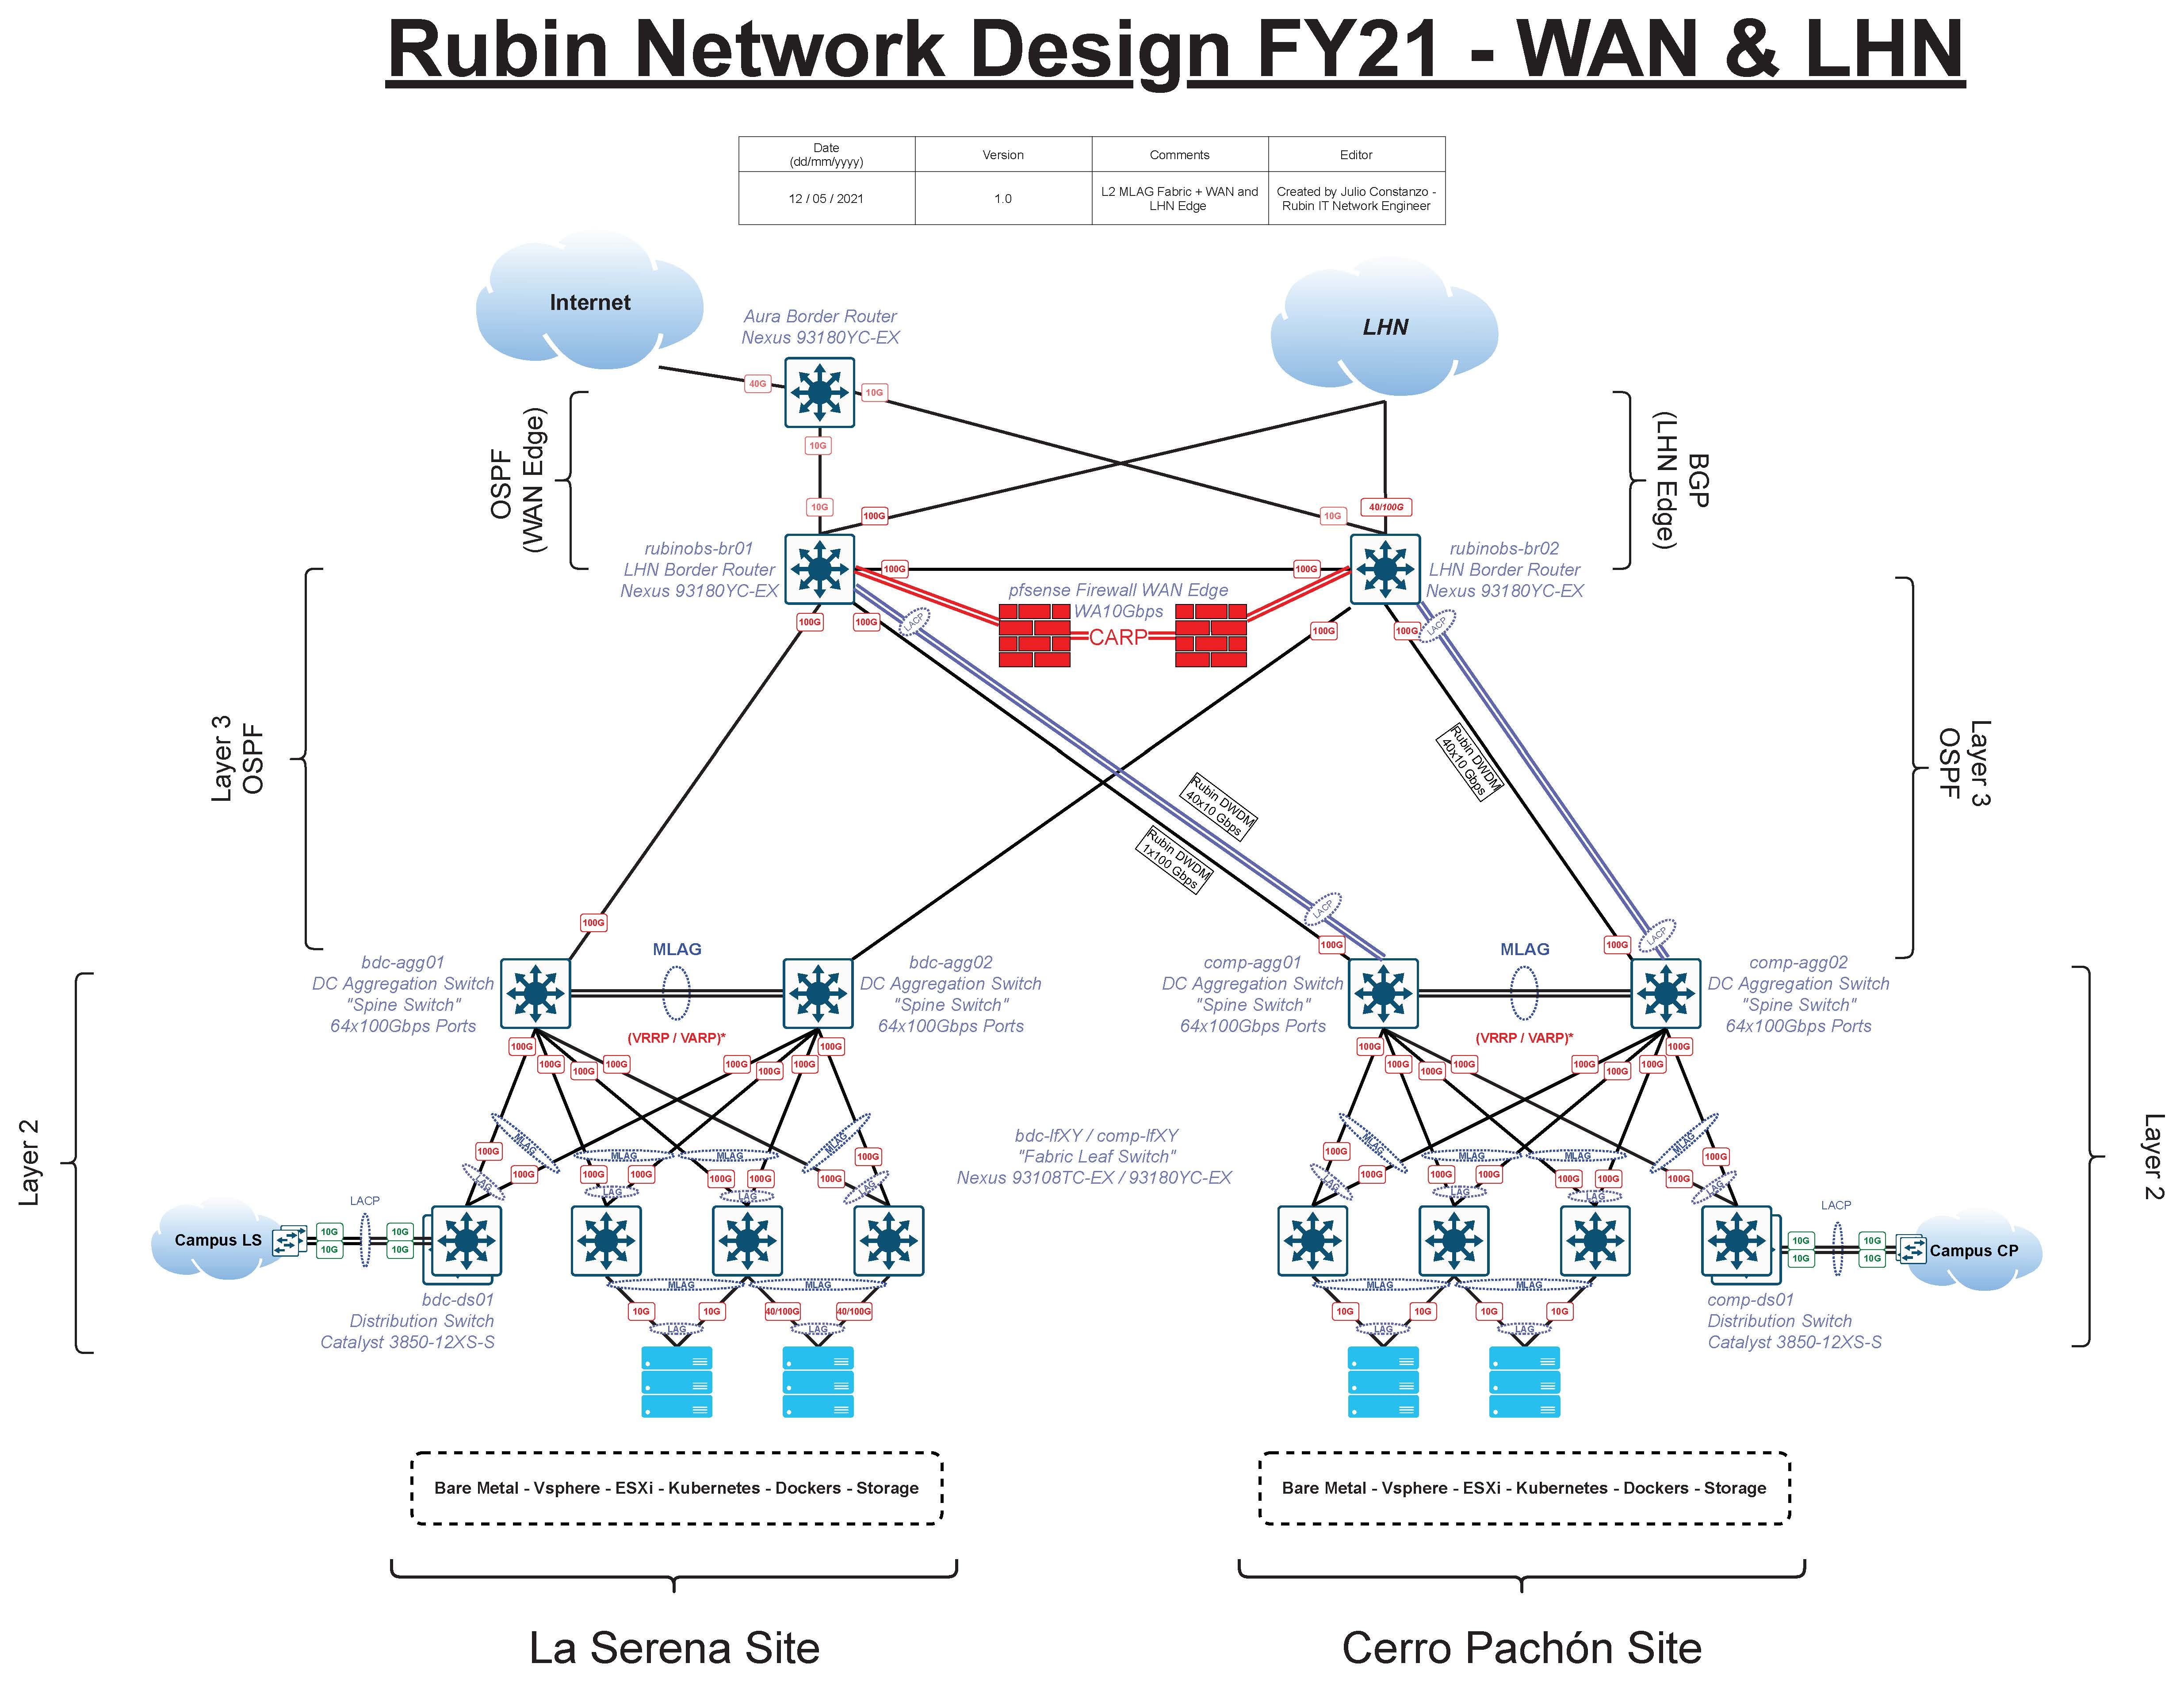
\includegraphics[width=15cm]{images/fy21-rubin-network.jpg}
    \centering
    \caption{FY21 Rubin Network Re-Design}
  \end{figure}

\newpage
\section{Arista}
\section{Cisco}

\subsection{Introduction}

Cisco Systems is an industry leader who develops, manufactures and sells networking hardware, software, telecommunications equipment and other high-technology services and products. 

Cisco NX-OS nowadays is a  well-known network operating system in the market with a good amount of documentation, provider and partner support around the globe, and dedicated forums to access in order to seek knowledge alongside officials’ courses and certifications. Cisco NX-OS is also well known for being a data center-class operating system that includes the following feature and benefits:

For features and benefits go to \href{https://www.cisco.com/c/en/us/products/collateral/ios-nx-os-software/nx-os-software/data_sheet_c78-652063.pdf}{Cisco-NXOS-DataSheet}

The quotations made by Cisco partner, NTT Chile can be found on confluence under: \href{https://confluence.lsstcorp.org/display/IT/ITTN-043+-+Rubin+Network+Re-Engineering}{ITTN-043 Resources - Quotation}

\subsection{Hardware}

Our actual data center network is based on Cisco hardware and ACI-oriented, the following image is a summary of summit and base actual ACI infrastructure:
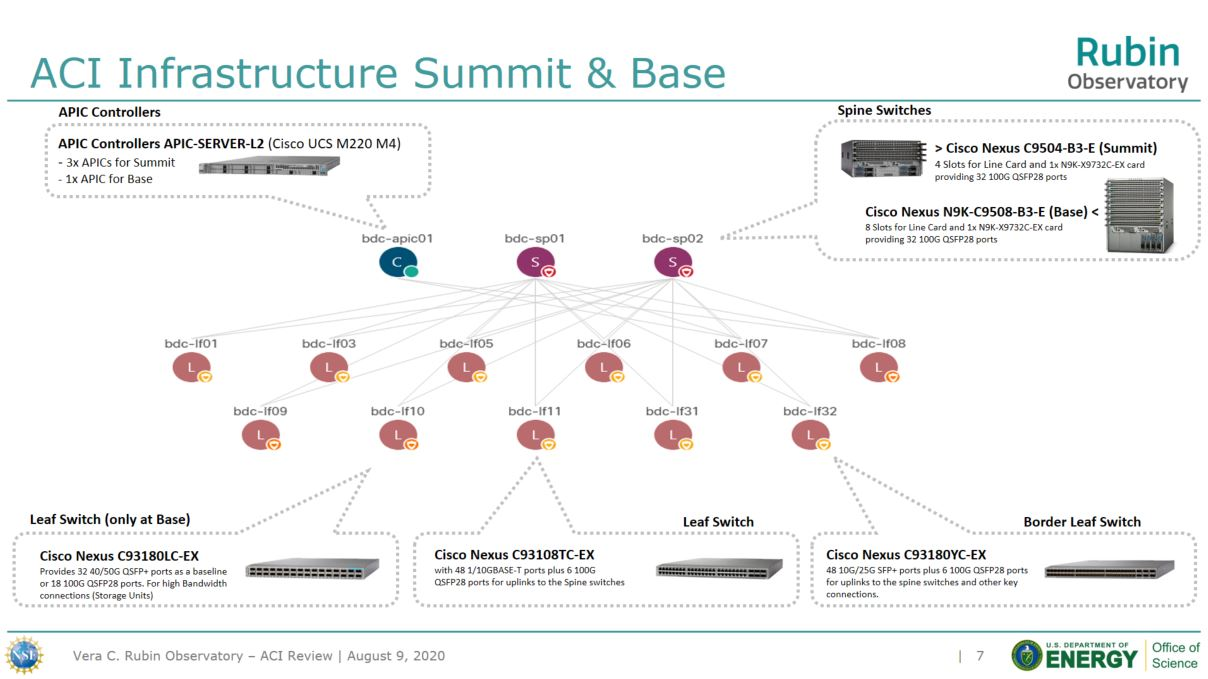
\includegraphics[width=10cm]{images/aci-infrastructure-summit-and-base.jpg}{Actual ACI Hardware Infrastructure Summit and Base}

The leaves switches can be migrated into NXOS since the software cames from fabric, we require to migrate the spine switches to NXOS. For that we have two options:

\begin{itemize}
    \item Option 1: Adquire NXOS software and licensing for spines switches, or
    \item Option 2: Adquire new spine switches for summit and base 
\end{itemize}

The hardware required in any case will be the already in place which is:

\begin{itemize}
    \item Summit: 2 units - Cisco Nexus C9504-B3-E - 4 Slots for Line Card and 1x N9K-X9732C-EX card providing 32 100G QSFP28 ports
    \item Base: 2 units - Cisco Nexus N9K-C9508-B3-E - 8 Slots for Line Card and 1x N9K-X9732C-EX card providing 32 100G QSFP28 ports
\end{itemize}

 
\subsection{License}

In order to go from ACI fabric to NX-OS, we were informed by Cisco and NTT that our leaves switches will require no further licensing since they came with NX-OS supported from fabric, but that was not the case for all the spine switches, who will require new licensing to support NX-OS when migrating from ACI operating system.

Quotations were requested to Cisco/NTT for NX-OS Essentials software licenses for both spine switches models (C9504 and C9508). Quotes can be found here: \href{https://confluence.lsstcorp.org/display/IT/ITTN-043+-+Rubin+Network+Re-Engineering?preview=/151855733/156506276/quote_nxos_licenses_march2021.pdf}{NXOS-Essential-Licenses}

\subsection{Network Design}

The network design is based on open-source protocols in order to avoid propietary protocols that could tied the network to an specific brand. The network design agreed by Rubin's IT Team is based first on NX-OS operating system, but using an MLAG aggregation core as spine switches, building a big layer 2 fabric at summit and base. 

The following topology explain on a high level design how the entire Rubin's network will look like:

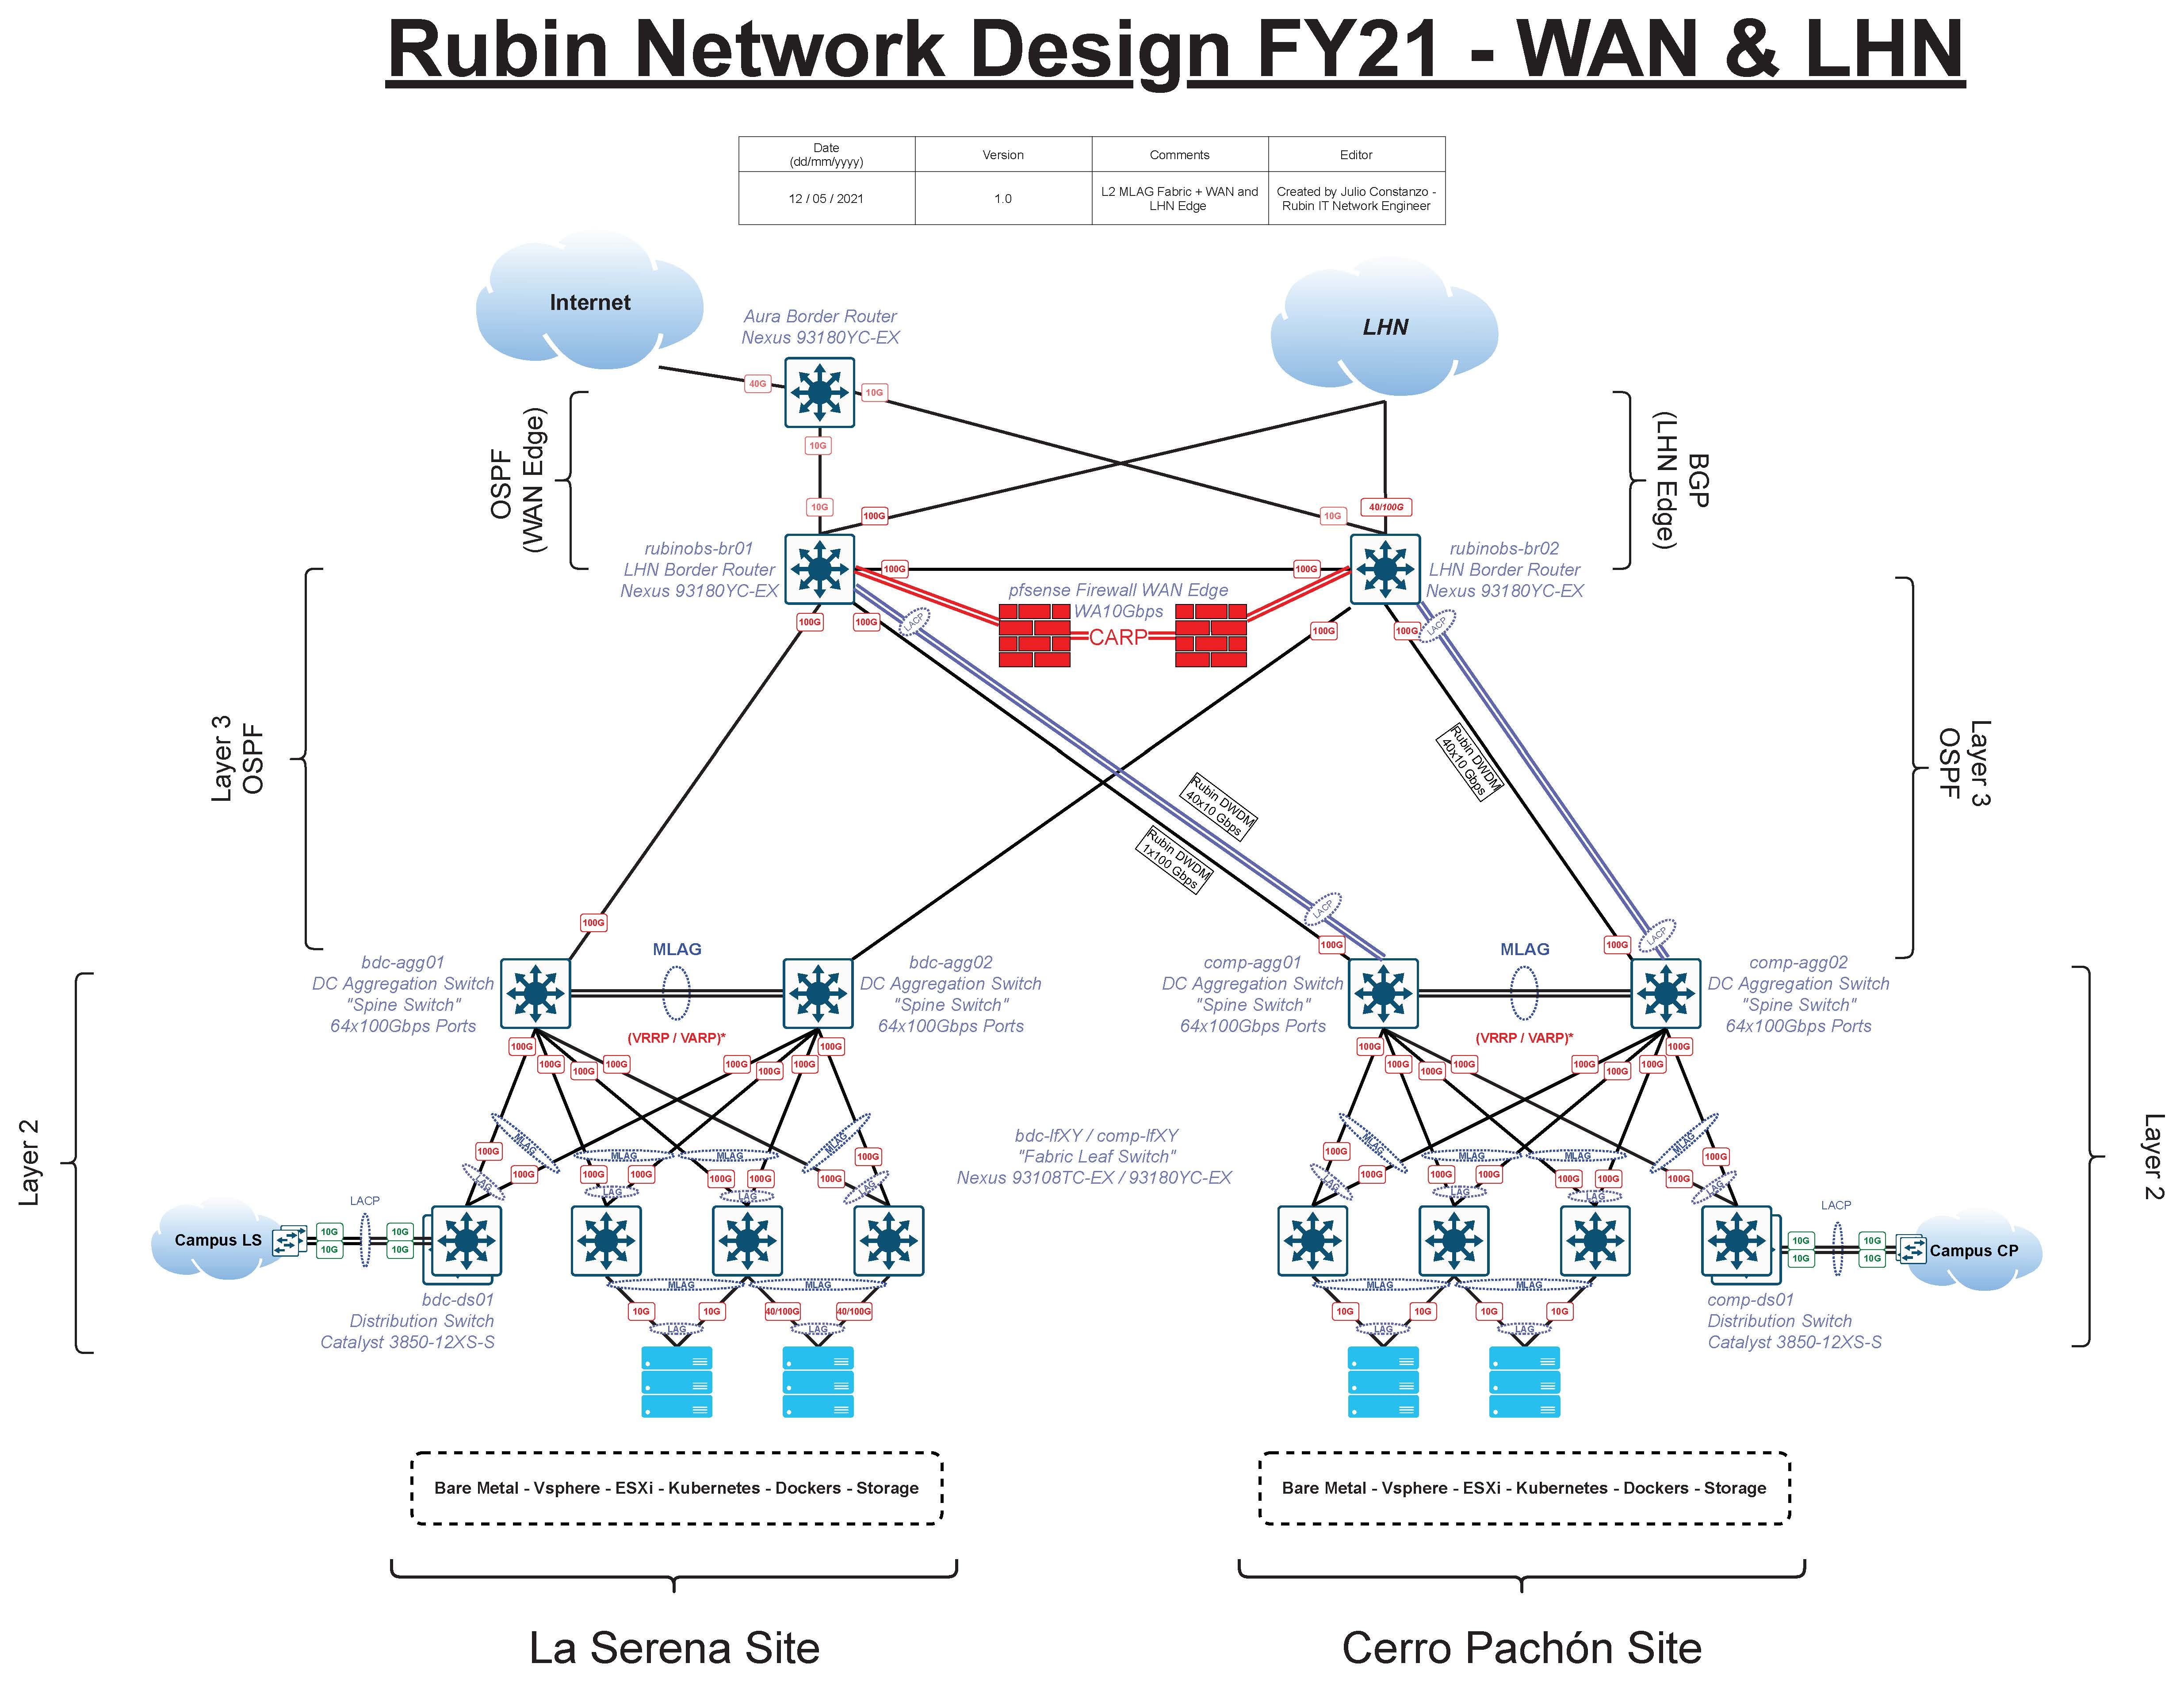
\includegraphics[width=15cm]{images/fy21-rubin-network.jpg}

\subsection{Support}

All quotation were requested and made with a 5-year support contract (8x5xNBD). Cisco also provides their specialist via Cisco TAC (Cisco Technical Assitance Center) which provides technical support to customers, partners and resellers.

Cisco provides two types of support:

\begin{itemize}
    \item Online at Cisco TAC website \href{http://www.cisco.com/tac}{Cisco TAC website}
    \item Via email/phone through the TAC Escalation Center
\end{itemize}

\subsection{Training}

Cisco is well known for having a large amount of certifications paths in the market, who are also well valued by enterprises around the globe. Most, if not all of them, have Cisco certifications paths into their training curses because of their market recognition. 

For more information about training and certifications please visit https://www.cisco.com/c/en/us/training-events/training-certifications/certifications/associate/ccna.html

\subsection{Pros/Cons}
\subsubsection{Pros}
\subsubsection{Cons}
\subsection{Closing Comments}

\section{Juniper}

\subsection{Introduction}
\subsection{Hardware}
\subsection{Software}
\subsection{Network Design}
\subsection{Support}
\subsection{Training}
\subsection{Pros}
\subsection{Cons}
\subsection{Closing Comments}
\section{Comparison Matrix}

The following is a summary comparison of the vendors.

\begin{figure}
    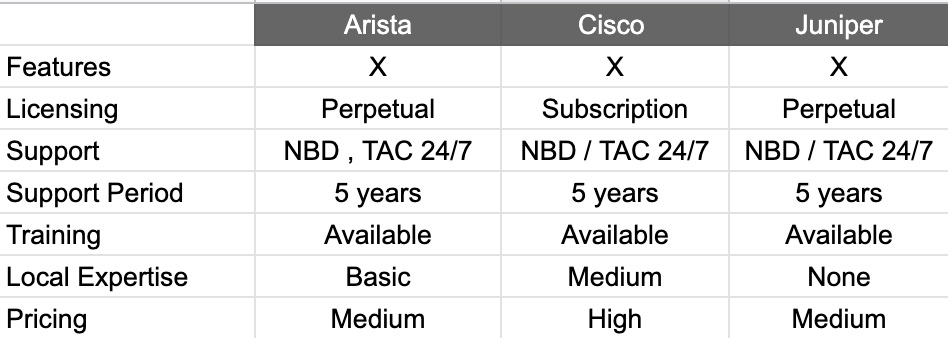
\includegraphics[width=11cm]{images/matrix.jpg}
    \centering
\end{figure}

All vendors met the technical requirements exposed in the network design. 

Cisco is the only vendor not offering a perpetual license; hence Cisco licenses must be renewed. 

Training is available for all vendors, but Juniper bundles an "All-Access Pass" for a year for a single person.

IT staff has plenty of experience with Cisco devices. Despite only a couple of Arista devices installed in Rubin's network, the expertise of Cisco can be extended to Arista, given that the interfaces are pretty similar. Regarding Juniper, Rubin Network engineers have no experience with it. 

Pricing details can be reviewed for each vendor; however, Cisco is the most expensive of them. 

All vendors offered five years of support which leaves Rubin well into operations. 


\section{Conclusion}

All vendors provide quality hardware and meet the technical requirements of Rubin IT's design. However, support, licensing, and experience with the products are essential factors that have to be considered in the final recommendation. 

\subsection{Support}
The team doesn't have good experiences with Cisco support. It has been challenging to talk with a Cisco Engineer, and going through the vendor has sometimes complicated more the issues. It is clear that after speaking with a Cisco Engineer, the flow of the communication improves, and problems are solved in a reasonable time. 

There's no experience with Arista and Juniper support, however, during the evaluation of the vendors, both provided access to virtual labs and engineers to discuss our design. It is the expectation that both vendors will behave similarly to our experience with Cisco Engineers. 

\subsection{License}
Cisco has shifted its licensing scheme to a subscription-based. This means that software licenses have to be renewed every few years, increasing the cost of equipment ownership and creating uncertainty for budget planning. There are also changes in features provided, hence there's no clarity if the current license tier will cover the needs of the network.

Arista and Juniper provide perpetual licensing.

\subsection{Experience}
Rubin IT and Noirlab engineers have plenty of experience with Cisco devices and little experience with Arista; however, given the similarity of the operating systems of both vendors, the Arista learning curve is relatively small. On the other hand, Juniper has an entirely different configuration structure based on commits, which could be beneficial in some cases but represents a much higher learning curve. 

\subsection{Recommendation}

Given this evidence, the best path is to migrate the Cisco ACI platform to a non-vendor locking technology based on Arista switches. 

Arista represents a small learning curve for Rubin and Noirlab engineers, provides all the features needed for the project, is competitively priced, and offers a better cost of ownership given its perpetual licensing model. 
The technology will be not be bound to a vendor, so unlike the current state, there will be a mix of vendors in the network, allowing Rubin to select the best available solution regardless of the vendor. 

The complexity of the network will be severely reduced, facilitating the troubleshooting of problems and increasing the time on sky.

Arista also has considerably fewer vulnerabilities reported in the last seven years. Cisco accounts for 2500 vulnerabilities, Juniper 300 and Arista 14. This is an essential factor to consider because each vulnerability, depending on its severity, could mean patching to the network equipment and potential interruptions or outages. It also brings up the topic of the quality of each vendor's software; it is clear that for Arista, security is an important.

The migration to Arista still needs to be analyzed and scheduled and will be laid out in a separate document. 

\appendix
% Include all the relevant bib files.
% https://lsst-texmf.lsst.io/lsstdoc.html#bibliographies
\section{References} \label{sec:bib}
\renewcommand{\refname}{} % Suppress default Bibliography section
\bibliography{local,lsst,lsst-dm,refs_ads,refs,books}

% Make sure lsst-texmf/bin/generateAcronyms.py is in your path
\section{Acronyms} \label{sec:acronyms}
\addtocounter{table}{-1}
\begin{longtable}{p{0.145\textwidth}p{0.8\textwidth}}\hline
\textbf{Acronym} & \textbf{Description}  \\\hline

AI & Artificial Intelligence \\\hline
ALMA & Atacama Large Millimeter Array (ESO) \\\hline
BGP &  Border Gateway Protocol \\\hline
BSR & Business Systems Review \\\hline
CVE & Common Vulnerabilities and Exposures \\\hline
EOS & Engineering Operations Services \\\hline
ESO & European Southern Observatory \\\hline
FY21 & Financial Year 21 \\\hline
IT & Information Technology \\\hline
L2 & Lens 2 \\\hline
LAN & Local Area Network \\\hline
LHN & long haul network \\\hline
NCSA & National Center for Supercomputing Applications \\\hline
NOIRLab & NSF's National Optical-Infrared Astronomy Research Laboratory; \url{https://nationalastro.org} \\\hline
NSF & National Science Foundation \\\hline
OS & Operating System \\\hline
PMO & Project Management Office \\\hline
TAC & Arista Global Technical Assistance Center \\\hline
US & United States \\\hline
\end{longtable}

% If you want glossary uncomment below -- comment out the two lines above
%\printglossaries





\end{document}
